
\documentclass[a4paper]{article}
\usepackage[margin=2cm]{geometry}

% --- FIX 1: Use fontspec for modern fonts and UTF-8 support with lualatex ---
\usepackage{fontspec}
% Latin Modern is a great default with excellent Unicode coverage but not good enough ...
\setmainfont{Latin Modern Roman}

% Set the monospaced font (used by \texttt and listings) to one
% with better Unicode character coverage, like DejaVu Sans Mono.
\setmonofont{DejaVu Sans Mono} % For \texttt and listings

\usepackage{graphicx}
\usepackage{xcolor}
\usepackage{listings}
\usepackage{hyperref}

\lstset{
    basicstyle=\ttfamily\small,
    breaklines=true,
}

\begin{document}
\title{Simulation Run Summary}
\author{Contiki-NG RPL Project}
\maketitle


\section*{Simulation Run: 20250818124554}
\subsection*{Source: \texttt{text\_20250818124554.txt}}

\begin{tabular}{@{}ll}
\textbf{Start Time:} & Mon Aug 18 2025 12:45:54 GMT+1200 (NZST) \\
\textbf{Finish Time:} & 18 Aug 12:48 \\
\textbf{Mode of Op:} & \texttt{N/A} \\
\textbf{Objective Funcs:} & \texttt{N/A} \\
\end{tabular}

\subsection*{Final Topology Summary}
\begin{lstlisting}
 DAG: fd00 (OF: OF0)
└── Root: 9
├── 1
├── 10
├── 11
├── 12
├── 15
├── 17
├── 18
├── 2
├── 20
├── 22
├── 23
├── 3
└── 4
 DAG: fd02 (OF: OF0)
└── Root: 9
├── 1
├── 10
├── 11
├── 12
├── 15
├── 18
├── 2
├── 20
├── 22
├── 23
├── 3
└── 4
└── 17
\end{lstlisting}

\subsection*{Visual Topology}
\begin{figure}
    \centering
    \begin{minipage}{0.48\textwidth}
        \centering
        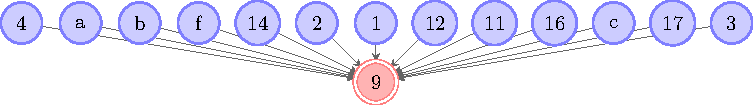
\includegraphics[page=1, width=\textwidth, trim=0 1cm 0 1cm, clip]{/home/stevecos/data/graph_20250818124554.pdf}
        \caption*{DODAG 1}
    \end{minipage}
    \hfill
    \begin{minipage}{0.48\textwidth}
        \centering
        \includegraphics[page=2, width=\textwidth, trim=0 1cm 0 1cm, clip]{/home/stevecos/data/graph_20250818124554.pdf}
        \caption*{DODAG 2 (if present)}
    \end{minipage}
\end{figure}

\hrule
\clearpage
\end{document}
